\chapter{Installation}
\section{Python}
Um dieses Tutorial durchführen zu können muss zuerst die Entwicklungsumgebung aufgesetzt werden. Als Programmiersprache wird in diesem Tutorial Python zum Einsatz kommen. Python gilt als höhere Programmiersprache die besonders auf kurzen und  gut lesbaren Programmierstil setzt. Charakteristisch ist zum Beispiel das Nichtverwenden von geschwungenen Klammern um Blöcke zu kennzeichnen. Diese werden in Python durch Einrückungen gekennzeichnet.\\
In diesem Tutorial wird die Python Version 3.6.5 oder höher verwendet. Diese muss, falls noch nicht installiert, von der offizielen Website \href{https://www.python.org}{https://www.python.org} heruntergeladen werden. Es gibt von Python sowohl eine Windows, MacOS als auch eine Linux Version. Je nach Betriebssystem sollte die richtige Version verwendet werden. Hat man den Installer heruntergeladen kann er auch einfach ausgeführt werden, wodurch dann Python installiert wird. Wichtig für die Windows Version ist hierbei, dass Python zu den Umgebunsvariablen hinzugefügt werden muss. Dies wird aber bei der Installation nachgefragt und kann bzw. sollte ausgewählt werden. Vergisst man dies, muss man Python manuell den Umgebunsvariablen hinzufügen.\\
Hat man Python installiert kann man überpüfen ob die Installation erfolgreich war. Dazu öffnet man einfach die Kommandozeile bzw. das Terminal und gibt bei Windows den Befehl \emph{python} bzw. bei MacOS und Linux den Befehl \emph{python3} ein. Dann sollte eine ähnliche Ausgabe wie bei Bild \ref{fig:cmd} ausgegeben werden. Im weiteren Verlauf dieses Tutorials wird nur noch der Befehl \emph{python3} verwendet. Windows Nutzer müssen aber im fortlaufenden Tutorial trotzdem \emph{python3} verwenden
\begin{figure}[!ht]
\centering
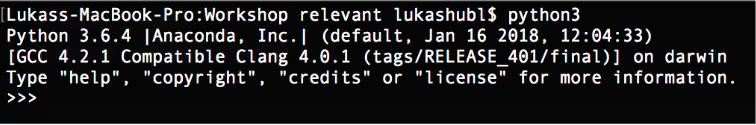
\includegraphics[width=1.00\textwidth]{images/cmd}
\caption{Ausgabefenster Kommandozeile bzw. Terminal bei erfolgreicher Installation}
\label{fig:cmd}
\end{figure}
\section{Pandas und Matplotlib}
Als nächstes werden zwei python Packages zum Visualisieren von Daten benötigt. Diese Packages können mit dem in Python integrierten Paketverwaltungsprogramm pip heruntergeladen und automatisch installiert werden. Das erste Package ist Pandas und kann mit dem Befehl \emph{pip install pandas} von der Kommandozeile bzw. vom Terminal aus installiert werden. Genau gleich kann man das Package Matplotlib installieren, nämlich mit dem Befehl \emph{pip install matplotlib}.\\
\section{Tensorflow}
Ähnlich verhält es sich mit der Installation unseres eigentlichen Frameworks Tensorflow. Dies kann auch mit pip heruntergeladen und installiert werden. Dazu muss der Befehl \emph{pip install tensorflow} auf der Kommandozeile bzw. auf dem Terminal ausgeführt werden. Dadurch wurde die Standardversion von Tensorflow installiert. Das bedeutet ohne GPU Unterstützungen und ohne bestimmte prozessorspezifische Instruktionen wie AVX2.\\
Um zu testen ob Tensorflow und alle Packages richtig installiert wurden, wurde ein Skript geschrieben welches alles Packages testet. Dafür muss vom Workshop-Repository das Skript \emph{setupCheck.py} heruntergeladen werden. Wird das Skript mit dem Befehl \emph{python3 setupCheck.py} ausgeführt gibt das Skrip aus ob die Entwicklungsumgebung mit allen Packages richtig installiert wurde. Die Ausgabe des ausgeführten Skripts sollte dann der Ausgabe des Bildes \ref{fig:setupCheck} ähneln.
\begin{figure}[!ht]
\centering
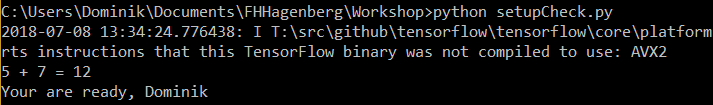
\includegraphics[width=1.00\textwidth]{images/setupCheck}
\caption{Ausgabefenster bei erfolgreichen ausführend des Skripts \emph{setupCheck.py}}
\label{fig:setupCheck}
\end{figure}
\section{Optional: Openvc}
Das Package \emph{opencv-python} wird später in unserer Realtime Klassifizierung benötigt um mit der Kamera des Notebooks oder PCs zu interagieren. Theoretisch gehört dieses package aber nicht zur Entwicklungsumgebung und wird deshalb hier als optional gekennzeichnet. Um die Realtime Klassifizierung programmieren bzw. ausführen zu können, wird dieses Package aber UNBEDINGT benötigt.\\
Das Package selsbt kann mit \emph{pip install opencv-python} installiert werden. Leider verhält es sich mit diesem Package anders als mit den anderen Packages und es enthält viele externe Abhängigkeiten zu anderen Packages. Da von PC zu PC unterschiedlich ist was bereits installiert ist und in unserem Fall relativ wenige Packages fehlten, können wir hier nicht angeben welche Packages nachinstalliert werden müssen. Ein Tipp ist es die Fehlermeldungen beim Ausführen des Codes zu betrachten und die fehlenden Packags mit pip nachinstallieren.\\
Dies wars dann auch mit der Installation der Entwicklungsumgebung.
\label{cha:Installation}